% SURROGATE MODELING
Another approach is to construct a global \emph{surrogate} or \emph{metamodel} of the simulator in the vein of a \emph{response surface} \cite{Statistics:Box2007,Statistics:Myers2016}.
The metamodel is built so as to emulate or mimic the behavior of the original model over its whole domain.
Typically it is cheap to evaluate and can therefore supersede the full model in analyses that require many model runs,
e.g.\ uncertainty propagation, sensitivity analysis and parameter estimation.
This renders the analysis of systems possible where using the simulator is ruled out due to the incurred computational cost.
Of course, this only works subject to the condition that the cost of computing a sufficiently accurate surrogate does not exceed the available budget either.
\par % METAMODELING TYPES
Widespread classes of metamodels are based on polynomial chaos expansions \cite{PCE:LeMaitre2010,PCE:Xiu2010},
Gaussian process models \cite{Kriging:Santner2003,Kriging:Rasmussen2006}, artificial neural networks \cite{ML:Bishop1995,ML:Ripley1996}
and support vector machines \cite{ML:Christmann2008,ML:Abe2010}.
Traditionally these emulator types have been developed and publicized in different scientific communities and disciplines.
While the two first-mentioned techniques are mainly used in engineering and statistics, respectively, the two last-mentioned ones are rooted in machine learning.
Nowadays they are used in a more cross-disciplinary and problem-oriented manner.
Polynomial chaoses \cite{PCE:Marzouk2007,PCE:Marzouk2009:a}, Gaussian processes \cite{Bayesian:Joseph2012,Bayesian:Joseph2013}
and neural networks \cite{ML:Raudensky1996,ML:Mares2016} are used in numerous different ways for parameter estimation.
Each approach certainly has its own advantages and the performance depends on the specific problem at hand.
One can combine different techniques in order to improve the efficiency \cite{Kriging:Kersaudy2015,Kriging:Schobi2015,PCE:Spiridonakos2015,PCE:Mai2016}.
\par % POLYNOMIAL CHAOS
In the following we concentrate on polynomial chaos--based metamodels.
Even though the theoretical foundations date back to the first half of the last century \cite{PCE:Wiener1938,PCE:Cameron1947},
this type of stochastic spectral expansion was popularized only during the last decades in the context of stochastic finite elements \cite{PCE:Ghanem1990,PCE:Ghanem1991}.
Technically speaking, a random variable is expanded with respect to a number of basis random variables.
We approach the topic from the perspective of function approximation \cite{Math:Rivlin1969,Math:DeVilliers2012}.
This matches more closely how the surrogate model is used after its construction in practice, i.e.\ it approximates function values for more or less arbitrarily chosen inputs.
\par % UNIVARIATE OUTPUT
We start with a scalar-valued model \(\mathcal{M} \colon \mathcal{D}_{\bm{x}} \rightarrow \mathds{R}\) as in \cref{eq:UQ:Simulator}.
It maps inputs \(\bm{x} \in \mathcal{D}_{\bm{x}}\) to outputs \(\tilde{y} = \mathcal{M}(\bm{x}) \in \mathds{R}\).
% MUTLTIVARIATE OUTPUT
In the vector-valued case one would treat each component separately.
Alternatively, one could make use of a non-canonical basis representation of the model output space and subsequently consider the coefficients individually.
This is further elaborated on in \cref{sec:Uncertainty:MultivariateOutput}.

\subsection{Spectral expansions}
% FUNCTION SPACE
Let us consider attractive spaces for the simulator.
Given a weight function \(w \colon \mathcal{D}_{\bm{x}} \rightarrow \mathds{R}^{+}\),
one may try to justify or simply assume that the model \(\mathcal{M} \in L_{w}^2(\mathcal{D}_{\bm{x}})\) belongs to the function space
\begin{equation} \label{eq:PCE:FunctionSpace}
  L_{w}^2(\mathcal{D}_{\bm{x}})
  = \left\{u \colon \mathcal{D}_{\bm{x}} \rightarrow \mathds{R} \cond \int\limits_{\mathcal{D}_{\bm{x}}} u^2(\bm{x}) \, w(\bm{x}) \, \mathrm{d} \bm{x} < \infty \right\}.
\end{equation}
% HILBERT SPACE
This is a Hilbert space with an inner product \(\langle \cdot,\cdot \rangle_w\) and an associated norm \(\lVert \cdot \rVert_w\).
For any two elements \(u,v \in L_{w}^2(\mathcal{D}_{\bm{x}})\) these are defined as
\begin{equation} \label{eq:PCE:ProductNorm}
  \left\langle u,v \right\rangle_w = \int\limits_{\mathcal{D}_{\bm{x}}} u(\bm{x}) v(\bm{x}) \, w(\bm{x}) \, \mathrm{d} \bm{x}, \quad
  \left\lVert u \right\rVert_w = \left\langle u,u \right\rangle_w^{1/2}.
\end{equation}
\par % BASIS EXPANSION
It now seems natural to seek for a Hilbert basis with respect to which one can expand vectors.
Let \(\{\basis_{i}\}_{i \in \mathds{N}_{>0}}\) be a complete orthonormal set of vector space elements \(\basis_{i} \in L_{w}^2(\mathcal{D}_{\bm{x}})\).
Thus for all \(i,j \in \mathds{N}_{>0}\) one has \(\langle \basis_{i}, \basis_{j} \rangle_w = \delta_{ij}\), where \(\delta_{ij}\) is the Kronecker delta.
As an element of the space in \cref{eq:PCE:FunctionSpace} the model can be expanded with respect to the orthonormal basis \(\{\basis_{i}\}_{i \in \mathds{N}_{>0}}\).
This so-called \emph{spectral expansion} is given as
\begin{align}
  \mathcal{M} &= \sum\limits_{i=1}^\infty \coeffM_{i} \basis_{i}, \label{eq:PCE:SpectralExpansion} \\
  \coeffM_{i} &= \langle \mathcal{M}, \basis_{i} \rangle_w. \label{eq:PCE:SpectralProjection}
\end{align}
\par % PROJECTION ONTO SUBSPACE
In practice one has to truncate the infinite series in \cref{eq:PCE:SpectralExpansion} and approximate it by a finite number of summands.
One therefore considers the projection of \(\mathcal{M}\) onto the subspace
\(\mathds{P}_P = \mathrm{span}(\{\basis_{i}\}_{i \leq P})\) spanned by the first \(P \in \mathds{N}_{>0}\) basis vectors \(\{\basis_{i}\}_{i \leq P}\).
This projection is given as
\begin{equation} \label{eq:PCE:SubspaceProjection}
  \mathcal{M}_P(\bm{x}) = \sum\limits_{i=1}^P \coeffM_{i} \basis_{i}(\bm{x}).
\end{equation}
% RESIDUAL VECTOR
The truncation error or residual \(r_P(\bm{x}) = \mathcal{M}(\bm{x}) - \mathcal{M}_P(\bm{x}) = \sum_{i=P+1}^\infty \coeffM_{i} \basis_{i}(\bm{x})\)
is orthogonal with respect to the subspace \(\mathds{P}_P \subset L_{w}^2(\mathcal{D}_{\bm{x}})\).
This means that \(\langle r_P, u_P \rangle_w = \langle u_P, r_P \rangle_w = 0\) for all \(u_P \in \mathds{P}_P\) which is denoted as \(r_P \, \bot \, \mathds{P}_P\).
One can characterize the residual in the respective Hilbert space norm.
The norm \(\lVert r_P \rVert_w\), or equivalently its square \(\lVert r_P \rVert_w^2 = \sum_{i=P+1}^\infty \coeffM_{i}^2\),
is minimized over the subspace \(\mathds{P}_P\) and converges to zero for \(P \to \infty\).
To make this explicit we write
\begin{equation} \label{eq:PCE:Optimality}
  \lVert r_P \rVert_w^2 = \operatorname*{inf}_{u_P \in \mathds{P}_P} \left\lVert \mathcal{M}-u_P \right\rVert_w^2, \quad
  \lim\limits_{P \to \infty} \lVert r_P \rVert_w^2 = 0.
\end{equation}
\par % GEOMETRIC INTERPRETATION
A geometric interpretation of the subspace projection in \cref{eq:PCE:SubspaceProjection} is provided in the familiar-looking \cref{fig:UQ:OrthogonalProjection}.
The model \(\mathcal{M} =  \coeffM_1 \basis_1 + \coeffM_2 \basis_2 + \coeffM_3 \basis_3\)
therein is an element of a three-dimensional function space \(\mathds{P}_3 = \mathrm{span}(\{\basis_1,\basis_2,\basis_3\})\).
Its projection onto the two-dimensional subspace \(\mathds{P}_2 = \mathrm{span}(\{\basis_1,\basis_2\})\)
is \(\mathcal{M}_2 = \coeffM_1 \basis_1 + \coeffM_2 \basis_2\).
The residual is simply the difference \(r_2 = \mathcal{M} - \mathcal{M}_2 = \coeffM_3 \basis_3\) between the true function and its approximation.
One has the orthogonality \(r_2 \, \bot \, \mathds{P}_2\).
% FIGURE: ORTHOGONAL PROJECTION
\begin{figure}[htbp]
  \centering
  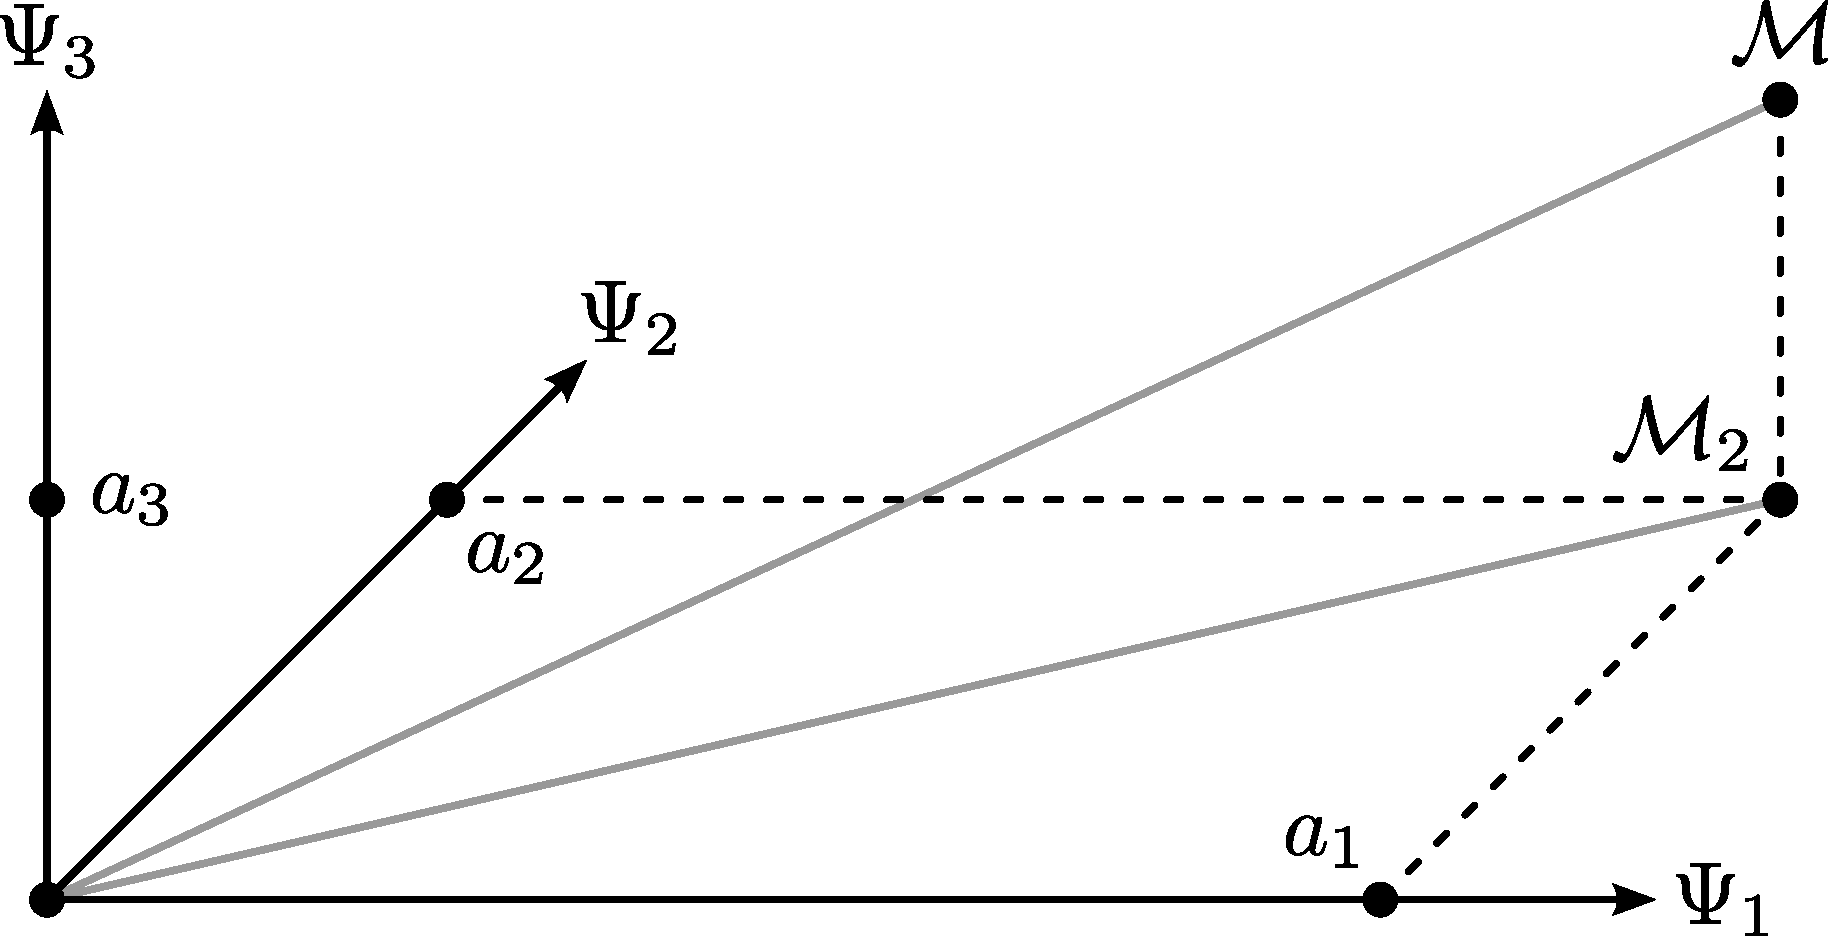
\includegraphics[width=7.7cm]{fig_UQ_OrthogonalProjection}
  \caption[Orthogonal projection]{Orthogonal projection.}
  \label{fig:UQ:OrthogonalProjection}
\end{figure}
\par % SECOND-ORDER RANDOM VARIABLES
In uncertainty analysis one often equates the positive weight function \(w(\bm{x}) = \pi(\bm{x})\) with the probability density of the inputs in \cref{eq:UQ:InputRV}.
This adds a probabilistic interpretation.
Elements \(u,v \in L_{\pi}^2(\mathcal{D}_{\bm{x}})\) define random variables \(u(\bm{X})\) and \(v(\bm{X})\) with finite variance.
The inner product in \cref{eq:PCE:ProductNorm} is an expectation value in the sense that \(\langle u, v \rangle_\pi = \mathds{E}[u(\bm{X}) v(\bm{X})]\).
By analogy with \cref{eq:PCE:SpectralExpansion}, the output in \cref{eq:UQ:OutputRV} can be expanded in terms of basis random variables \(\{\basis_{i}(\bm{X})\}_{i \in \mathds{N}_{>0}}\)
as \(\mathcal{M}(\bm{X}) = \sum_{i=1}^\infty \coeffM_{i} \basis_{i}(\bm{X})\).
This is called a \emph{stochastic spectral expansion} at times.

\subsection{Polynomial approximations}
% INDEPENDENT INPUTS
Now we assume that the random input variables are independent, i.e.\ their density factorizes into \(\pi(\bm{x}) = \pi_1(x_1) \ldots \pi_\dimParam(x_\dimParam)\).
% HILBERT SPACE TENSOR PRODUCT
The space \(L_{\pi}^2(\mathcal{D}_{\bm{x}}) = \{u \colon \mathcal{D}_{\bm{x}} \rightarrow \mathds{R} \cond \mathds{E}[u^2(\bm{X})] < \infty\}
\cong L_{\pi_1}^2(\mathcal{D}_{x_1}) \otimes \ldots \otimes L_{\pi_\dimParam}^2(\mathcal{D}_{x_\dimParam})\) is then isomorphic to the tensor product of the Hilbert spaces
\(L_{\pi_i}^2(\mathcal{D}_{x_i}) = \{u_i \colon \mathcal{D}_{x_i} \rightarrow \mathds{R} \cond \mathds{E}[u_i^2(X_i)] < \infty\}\) for \(i=1,\ldots,\dimParam\).
They have the inner products \(\langle u_i, v_i\rangle_{\pi_i} = \mathds{E}[u_i(X_i) v_i(X_i)]\) for \(u_i,v_i \in L_{\pi_i}^2(\mathcal{D}_{x_i})\).
For two elements \(u = u_1 \otimes \ldots \otimes u_\dimParam\) and \(v = v_1 \otimes \ldots \otimes v_\dimParam\) of the Hilbert space tensor product
one thus has \(\left\langle u,v \right\rangle_\pi = \left\langle u_1,v_1 \right\rangle_{\pi_1} \ldots \left\langle u_\dimParam,v_\dimParam \right\rangle_{\pi_\dimParam}\).
If the spaces \(L_{\pi_i}^2(\mathcal{D}_{x_i})\) have bases \(\{\basisU^{(i)}_{\alpha_i}\}_{\alpha_i \in \mathds{N}}\)
then \(\{\basisU^{(1)}_{\alpha_1} \otimes \ldots \otimes \basisU^{(\dimParam)}_{\alpha_\dimParam}\}_{\alpha_1,\ldots,\alpha_\dimParam \in \mathds{N}}\)
forms a basis of \(L_{\pi}^2(\mathcal{D}_{\bm{x}})\).
\par % ORTHOGONAL POLYNOMIALS
Before constructing a basis of \(L_{\pi}^2(\mathcal{D}_{\bm{x}})\) this way, convenient bases of the \(L_{\pi_i}^2(\mathcal{D}_{x_i})\) function spaces are discussed.
Polynomials that are orthogonal with respect to inner products whose weight function corresponds to common probability densities often constitute such bases.
Those polynomials are intimately related to the distributional moments.
% UNIVARIATE POLYNOMIALS
One starts by considering a family of polynomials \(\{\basisU_{\alpha_i}^{(i)}(x_i)\}_{\alpha_i \in \mathds{N}}\) in a single input variable \(x_i \in \mathcal{D}_{x_i}\).
Here, \(\alpha_i \in \mathds{N}\) is the polynomial degree.
The orthogonality relation is \(\langle \basisU^{(i)}_{\alpha_i}, \basisU^{(i)}_{\beta_i} \rangle_{\pi_i} = \delta_{\alpha_i \beta_i} \lVert \basisU^{(i)}_{\alpha_i} \rVert_{\pi_i}^2\).
% CLASSICAL FAMILIES
Four well-known distributions and their associated orthogonal polynomials are listed in \cref{tab:PCE:OrthogonalPolynomials}.
% UNIVARIATE LEGENDRE POLYNOMIALS
The uniform distribution is linked to the Legendre polynomials.
Their first six members \(\{P_\alpha(x)\}_{\alpha=0}^5\) up to degree five in a single variable \(x \in [-1,1]\) are shown in \cref{fig:UQ:LegendrePolynomials}.
% TABLE & FIGURE: STANDARD POLYNOMIALS
\begin{figure}[ht]
  \centering
  % TABLE: ORTHOGONAL POLYNOMIALS
  \begin{minipage}[c]{0.45\textwidth}
    \captionof{table}[Orthogonal polynomials]{Orthogonal polynomials.}
    \label{tab:PCE:OrthogonalPolynomials}
    \centering
    \begin{tabular}{lll}
      \toprule
      Distribution & Support & Polynomials \\
      \midrule
      Gaussian & \((-\infty,\infty)\) & Hermite  \\
      Uniform  & \([-1,1]\)           & Legendre \\
      Beta     & \([-1,1]\)           & Jacobi   \\
      Gamma    & \([0, \infty)\)      & Laguerre \\
      \bottomrule
    \end{tabular}
  \end{minipage}%
  % FIGURE: LEGENDRE POLYNOMIALS
  \begin{minipage}[c]{0.55\textwidth}
    \centering
    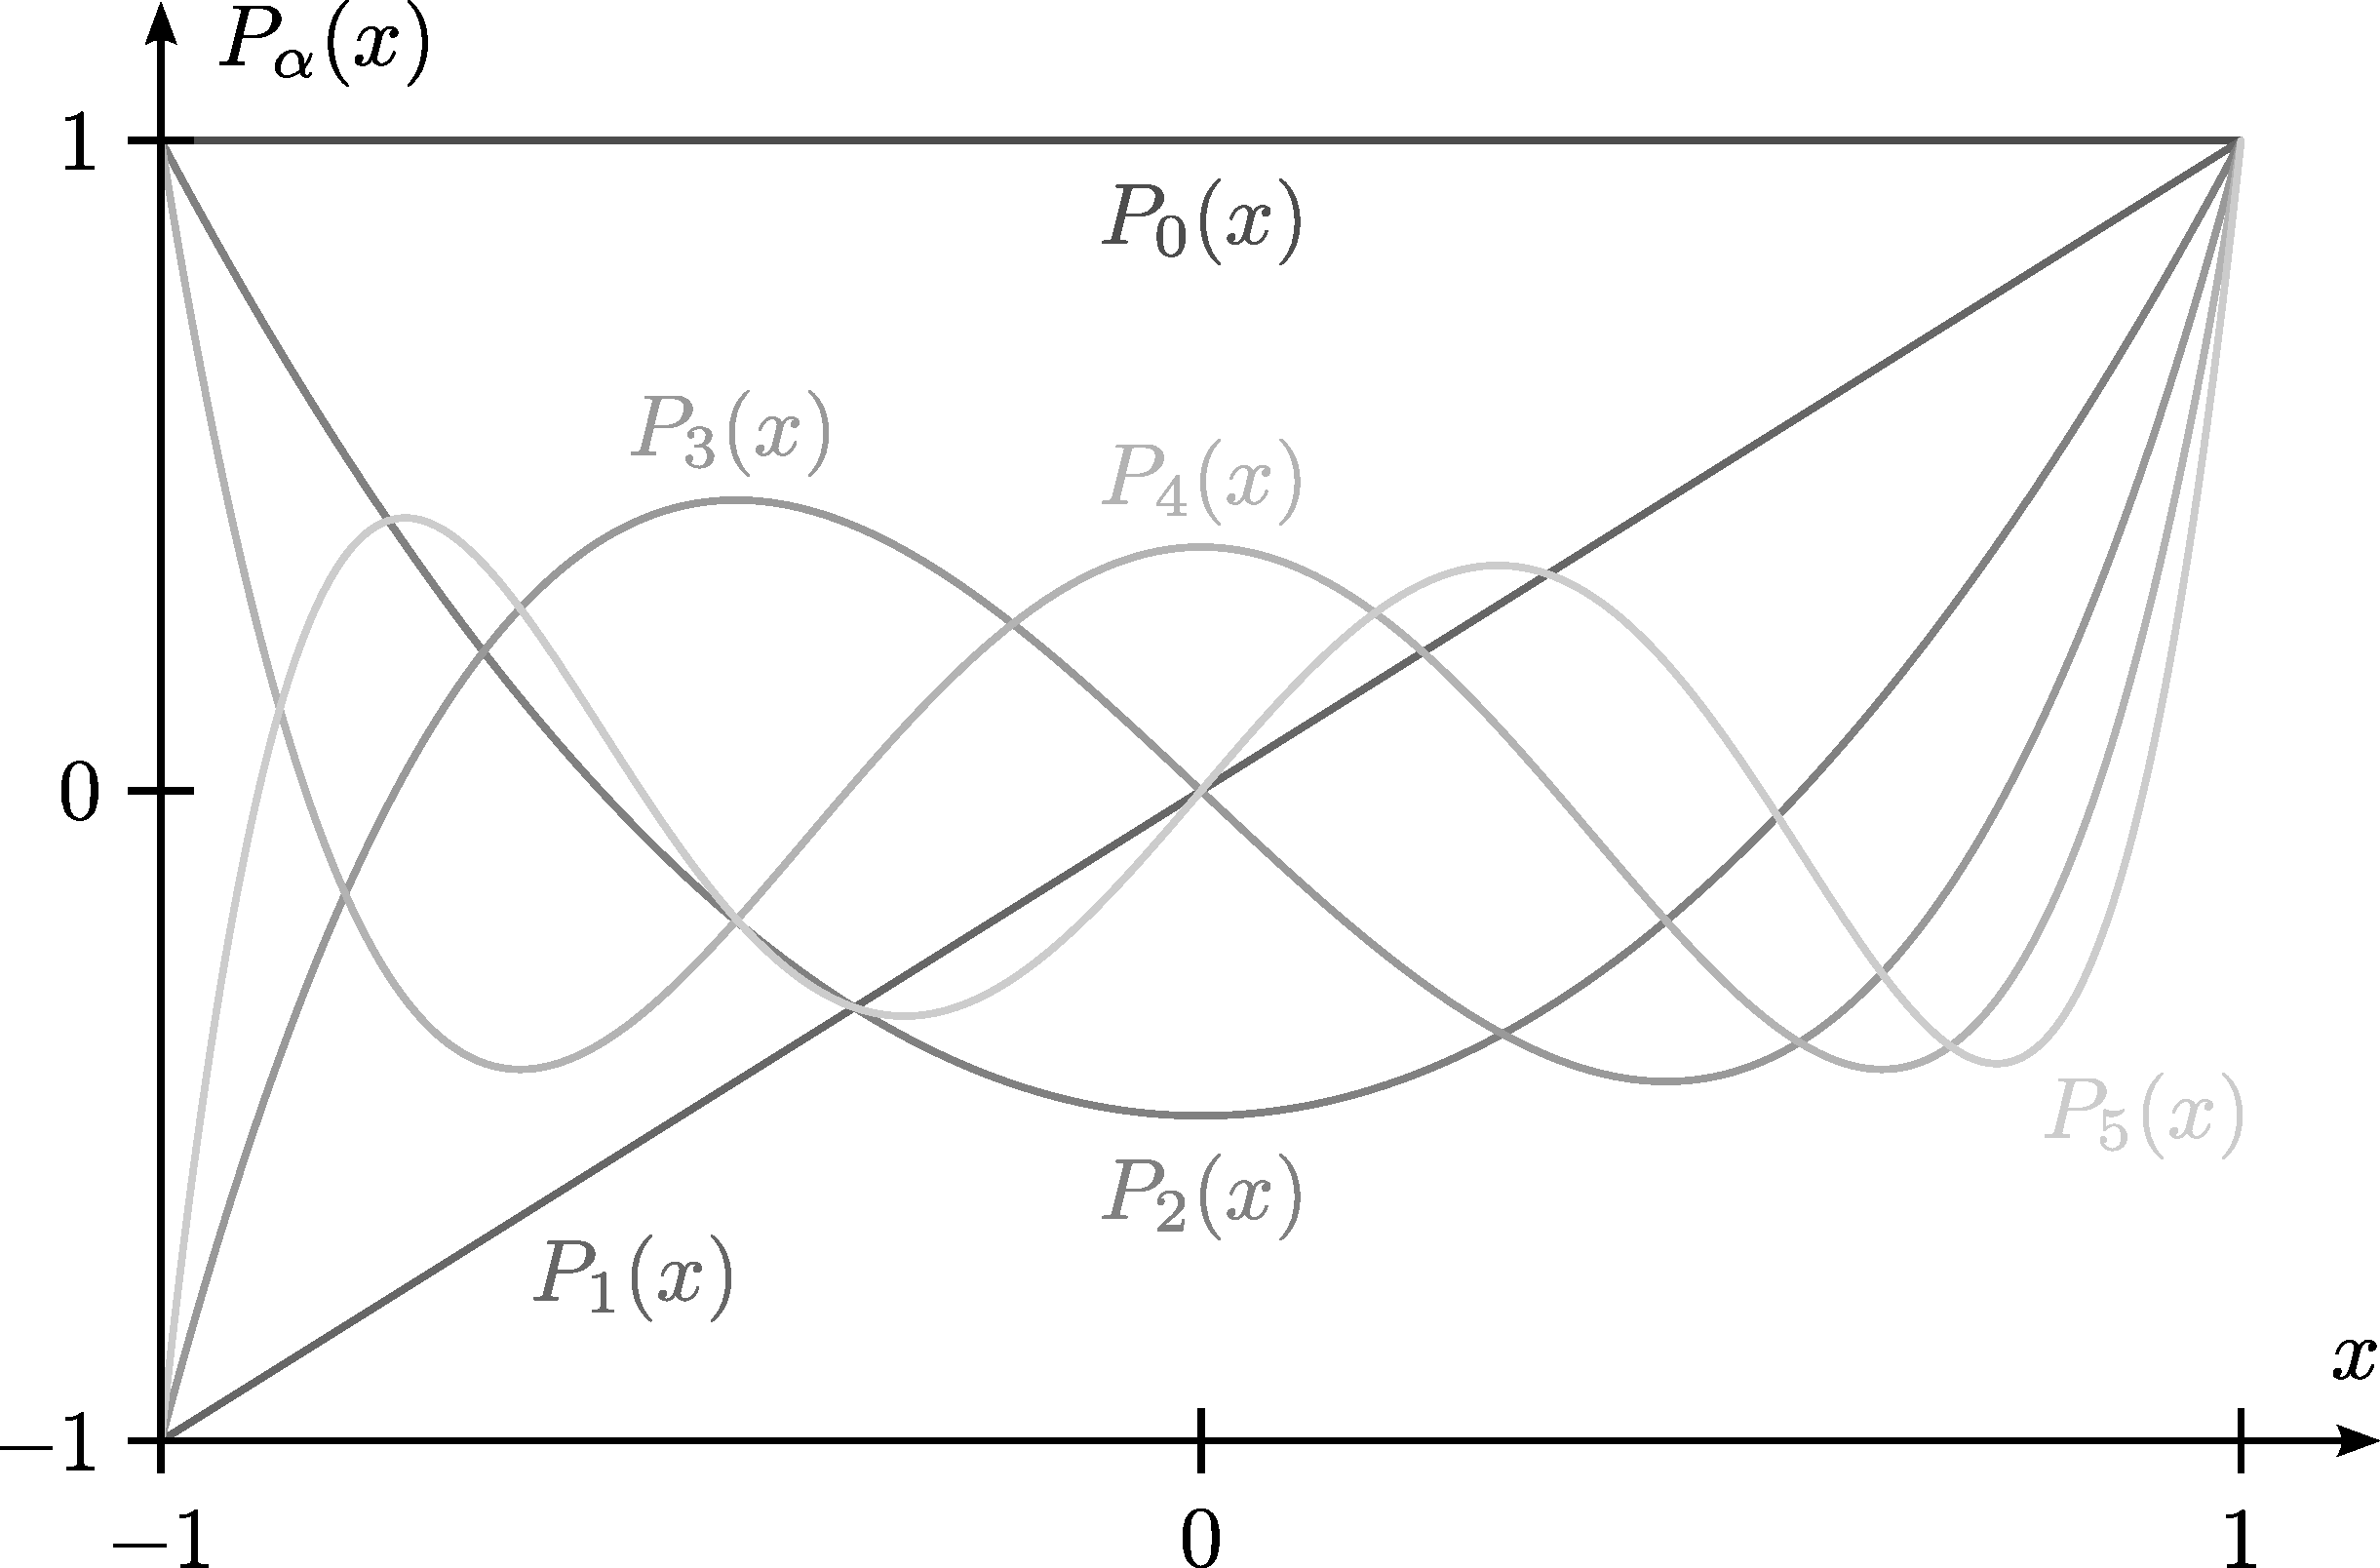
\includegraphics[width=8cm]{fig_UQ_LegendrePolynomials}
    \captionof{figure}[Legendre polynomials]{Legendre polynomials.}
    \label{fig:UQ:LegendrePolynomials}
  \end{minipage}%
\end{figure}
\par % COMPLETE SET
Such polynomials often constitute a complete set in \(L_{\pi_i}^2(\mathcal{D}_{x_i})\) \cite{PCE:Xiu2002:a,PCE:Xiu2002:b,PCE:Xiu2002:c}.
% LOGNORMAL DISTRIBUTION
A notable exception is the lognormal distribution for which one has to take care of some subtleties related to moment determinacy \cite{PCE:Ernst2012}.
This distribution is not uniquely determined by its sequence of moments, i.e.\ other genuinely different distributions feature the same moments.
The corresponding polynomials are not dense in the full space of mean-square integrable functions.
They form a set of elements that is orthogonal but not complete, i.e.\ \(\mathrm{span}(\{\basisU^{(i)}_{\alpha_i}\}_{\alpha_i \in \mathds{N}}) \subsetneq L_{\pi_i}^2(\mathcal{D}_{x_i})\).
Intuitively this becomes clearer by realizing that the linear hull of the polynomials is at most the intersection of different function spaces in which the polynomials are orthogonal.
\par % SUBSPACE RESTRICTION
In this situation one has to consider a slightly less general case,
e.g.\ mean-square integrability is replaced by the stronger assumption that the model is actually in the subspace spanned by the polynomials.
One may also argue that only the model's projection onto the respective subspace is considered in this case, i.e.\ the orthogonal complement is simply discarded.
Similar arguments can be evoked when constructing a finite number of polynomials that are orthogonal with respect to a distribution
that is empirically known by its first few moments only \cite{PCE:Witteveen2006:Proc,PCE:Oladyshkin2012,PCE:Ahlfeld2016}.
Another obvious possibility to bypass the problem is to transform the lognormal to a normal distribution by taking the natural logarithm.
\par % STANDARDIZED VARIABLES
Speaking of parameter transformations, it may very well be necessary to reparametrize the problem either way.
This happens so as to guarantee that the inputs have convenient bounds and probability distributions, e.g.\ the standard types that are compiled in \cref{tab:PCE:OrthogonalPolynomials}.
A related discussion on probabilistic model parametrizations is found in \cref{sec:Bayesian:ModelParametrization}.
Uniform distributions with arbitrary bounds can be linearly transformed into \(\pi_i(x_i) = \mathcal{U}(x_i \cond -1,1)\)
with \(\mathcal{U}(x_i \cond -1,1) = 1/2\) for \(x_i \in [-1,1]\) and \(\mathcal{U}(x_i \cond -1,1) = 0\) otherwise.
Similarly, Gaussians with arbitrary mean and variance can be shifted and scaled into a standard normal \(\pi_i(x_i) = \mathcal{N}(x_i \cond 0,1) = \exp(-x_i^2/2) / \sqrt{2\pi}\)
with mean \(\mu_{X_i} = 0\) and variance \(\sigma_{X_i}^2 = 1\).
We assume that our parameters are already of such a standard form.
\par % MULTIVARIATE POLYNOMIALS
Having univariate polynomials \(\{\basisU_{\alpha_i}^{(i)}(x_i)\}_{\alpha_i \in \mathds{N}}\) for each variable \(x_i\), multivariate polynomials in \(\bm{x}\) are constructed via tensorization.
We introduce a multi-index \(\bm{\alpha} = (\alpha_1,\ldots,\alpha_\dimParam) \in \mathds{N}^\dimParam\) for bookkeeping purposes.
Then a set of multivariate polynomials \(\{\basisU_{\bm{\alpha}}(\bm{x})\}_{\bm{\alpha} \in \mathds{N}^\dimParam}\) is given through
\begin{equation} \label{eq:PCE:MultivariatePolynomial}
  \basisU_{\bm{\alpha}}(\bm{x}) = \prod\limits_{i=1}^\dimParam \basisU^{(i)}_{\alpha_i}(x_i).
\end{equation}
In this construction, the orthogonality of the multivariate polynomials carries over from the univariate ones.
This is verified by
\(\langle \basisU_{\bm{\alpha}}, \basisU_{\bm{\beta}} \rangle_\pi = \delta_{\bm{\alpha} \bm{\beta}} \lVert \basisU_{\bm{\alpha}} \rVert_\pi^2
= \delta_{\alpha_1 \beta_1} \ldots \delta_{\alpha_\dimParam \beta_\dimParam}
\lVert \basisU^{(1)}_{\alpha_1} \rVert_{\pi_1}^2 \ldots \lVert \basisU^{(\dimParam)}_{\alpha_\dimParam} \rVert_{\pi_\dimParam}^2\).
\par % POLYNOMIAL EXPANSION
The polynomials defined in \cref{eq:PCE:MultivariatePolynomial} are complete in \(L_{\pi}^2(\mathcal{D}_{\bm{x}})\).
In the vein of \cref{eq:PCE:SpectralExpansion,eq:PCE:SpectralProjection}, the expansion of the model with respect to the multivariate polynomial basis
\(\{\basisU_{\bm{\alpha}}(\bm{x})\}_{\bm{\alpha} \in \mathds{N}^\dimParam}\) is given as
\begin{align}
  \mathcal{M} &= \sum\limits_{\bm{\alpha} \in \mathds{N}^\dimParam} \coeffM_{\bm{\alpha}} \basisU_{\bm{\alpha}}, \label{eq:PCE:PolynomialExpansion} \\
  \coeffM_{\bm{\alpha}} &= \langle \mathcal{M}, \basisU_{\bm{\alpha}} \rangle_\pi / \lVert \basisU_{\bm{\alpha}} \rVert_\pi^2. \label{eq:PCE:PolynomialCoefficient}
\end{align}
The stochastic spectral version of \cref{eq:PCE:PolynomialExpansion,eq:PCE:PolynomialCoefficient} is a certain \emph{polynomial chaos expansion} (PCE)
\(\tilde{Y} = \mathcal{M}(\bm{X}) = \sum_{\bm{\alpha} \in \mathds{N}^\dimParam} \coeffM_{\bm{\alpha}} \basisU_{\bm{\alpha}}(\bm{X})\) of the random variable in \cref{eq:UQ:OutputRV}.
Note that one can normalize the basis elements \(\{\basisU_{\bm{\alpha}}\}_{\bm{\alpha} \in \mathds{N}^\dimParam}\)
and linearly order them according to their multi-index \(\bm{\alpha}\).
\par % TRUNCATION SCHEME
An ordering scheme of some type can also facilitate the truncation of the series in \cref{eq:PCE:PolynomialExpansion} as in \cref{eq:PCE:SubspaceProjection}.
In a quite natural way one can impose restrictions on the total degree
\(\lVert \bm{\alpha} \rVert_1 = \sum_{i=1}^\dimParam \lvert \alpha_i \rvert\) of the polynomials in \cref{eq:PCE:MultivariatePolynomial}.
A finite number of terms is obtained by keeping only the ones with a total degree equal to or smaller than a certain \(p \in \mathds{N}\).
These are the terms indexed by \(\bm{\alpha} \in \mathcal{A}_p\) in \(\mathcal{A}_p = \left\{ \bm{\alpha} \in \mathds{N}^\dimParam \colon \lVert \bm{\alpha} \rVert_1 \leq p \right\}\).
The cardinality \(P\) of this set is dependent on the input dimensionality \(\dimParam\) and the maximal degree \(p\) through
\begin{equation} \label{eq:PCE:Cardinality}
  P = \begin{pmatrix}
        \dimParam + p \\
        p \\
      \end{pmatrix}
    = \frac{(\dimParam + p)!}{\dimParam! \, p!}.
\end{equation}
% CURSE OF DIMENSIONALITY
The fast growth of the total number of terms \(P\) in \cref{eq:PCE:Cardinality} can be ascribed to the curse of dimensionality.
That issue is further discussed in \cref{sec:Uncertainty:CurseOfDimensionality}.
% POLYNOMIAL APPROXIMATION
By retaining only the terms \(\{\basis_{\bm{\alpha}}\}_{\bm{\alpha} \in \mathcal{A}_p}\) in the expansion
the best polynomial approximation of total degree \(p\) is given by
\begin{equation} \label{eq:PCE:TruncatedApproximation}
  \mathcal{M}_P = \sum\limits_{\bm{\alpha} \in \mathcal{A}_p} \coeffM_{\bm{\alpha}} \basis_{\bm{\alpha}}.
\end{equation}
\par % ADVANTAGES OF POLYNOMIALS
Using a polynomial basis has some appealing advantages.
In the first place it is easy to understand and interpret, e.g.\ the contributing terms can be classified according to their polynomial degrees and multivariate structure.
One can distinguish between low-order and high-order terms or identify individual contributions and mutual interactions of input variables.
Furthermore, one could argue that many physical laws and models lend themselves to polynomial approximations,
e.g.\ think about Taylor expansions as in \cref{sec:Uncertainty:TaylorApproximation}.
\par % STATISTICAL MOMENTS
For intents of uncertainty quantification it is convenient that the coefficients of polynomial expansions
are related to the statistical moments in \cref{eq:UQ:OutputMean,eq:UQ:OutputVariance}.
One has for instance
\begin{equation} \label{eq:PCE:OutputMeanVariance}
  \mu_{\tilde{Y}} = \coeffM_{\bm{0}} \lVert \basisU_{\bm{0}} \rVert_\pi, \quad
  \sigma_{\tilde{Y}}^2 = \sum_{\bm{\alpha} \in \mathds{N}^\dimParam  \setminus \{\bm{0}\}} \coeffM_{\bm{\alpha}}^2 \lVert \basisU_{\bm{\alpha}} \rVert_\pi^2.
\end{equation}
The constant expansion term determines the expected value \(\mu_{\tilde{Y}} = \mathds{E}[\mathcal{M}(\bm{X})]\) in \cref{eq:PCE:OutputMeanVariance}.
So do the remaining terms for the variance \(\sigma_{\tilde{Y}}^2 = \mathrm{Var}[\mathcal{M}(\bm{X})]\).